\chapter{Introduction}
In recent years, network representations of complex systems have been applied widely throughout many scientific disciplines, contributing statistical tools designed to aid in an understanding of intricate causal structures that drive the behavior of multivariate processes \cite{borgatti2009network,barabasi2016network}. For instance, network models---i.e., \textit{probabilistic graphical models} \cite{lauritzen1996graphical}---have been used by psychologists in studying such diverse phenomena as the dynamics of psychopathology \cite{cramer2010comorbidity,epskamp2018personalized}, personality development across the lifespan \cite{read2010neural,costantini2019stability}, the associative structure of words in memory \cite{hills2010associative,de2008word}, the role of probabilistic phonotactics in spoken word recognition \cite{vitevitch2016phonological}, and connections between social networks and personal well-being \cite{kindermann1980relation,galaskiewicz1993social}. Researchers working within these domains, among others, are often interested in characterizing the underlying structure that relates variables within a multivariate system, as well as the dynamic, interdependent connections that make up important links between psychological, sociological, and behavioral variables as they interact and change over time.

Although they have been applied to a wide array of topics, the general goal of psychological network modeling is to characterize the unique associations among variables that are theorized to be interrelated with regard to some psychological process or construct. These models have been applied within both cross-sectional and longitudinal contexts, where in the former the objective is often to describe which variables have conditional relationships across multiple individuals, and in the latter the goal is often to describe the evolution and development of these relationships within a single individual over time. Multilevel implementations of longitudinal models---termed temporal networks---have also been employed in the study of whether those within-person processes hold across groups of individuals \cite{epskamp2018gaussian,epskamp2018personalized}.

While psychological networks have been shown to have a variety of diverse applications, they are limited by the fact that they currently only consider pairwise relationships among sets of variables. Specifically, they don’t take into consideration more complex relational structures such as those characterized by moderation effects and higher-order interactions. Moderation analysis, which focuses on these types of effects, is a common technique used within psychological research to help reveal the \textit{contexts} and \textit{conditions} under which different relationships may emerge or be observed among variables. For instance, we may be interested in whether the relationship between anxiety and insomnia is dependent on the degree to which an individual is experiencing situational stress. It is well-known that moderators can be crucial for understanding conditional interdependencies between variables, and that failing to investigate such variables when they are present can lead to a distorted understanding of the underlying phenomenon. Thus, my goal for this research is to extend the psychological network framework to include moderator variables, as well as provide statistical tools and software to facilitate testing such models with psychological data. 

In this paper, I present some background and description of \textit{moderated network models} (MNMs), as well as how these have been implemented in a software package for R that I'm currently developing called \code{modnets}. I begin by presenting and describing different types of psychological network models, as well as how they are commonly interpreted in the literature. Next, I provide some background on moderated regression analysis, along with how to specify and interpret interaction terms within these models. Then I will introduce moderated network models and present some examples of cross-sectional networks using an example dataset. In this paper, my focus is restricted to cross-sectional networks in order to introduce the most basic form of MNMs. In a subsequent paper, I will introduce and further discuss \textit{moderated temporal networks}, as well as how to analyze them using functions in the forthcoming \code{modnets} package for R. 

\section{Psychological Networks}
It is an important goal for psychologists to develop and improve upon methods for describing complex relationships among observed variables. The dominant approach toward this end has long been \textit{latent variable modeling}, where the objective is to connect a set of observations with some unobserved latent construct(s) using methods such as confirmatory factor analysis and structural equation modeling \cite{little2006merits}. In general, these methods aim at highlighting the shared variance among variables while downplaying their conditional relationships. The \textit{network perspective} in psychology, however, offers a powerful counterpoint to this approach by framing psychological constructs as systems of interacting variables rather than manifestations of unobserved factors. Thus, while latent variable models are designed to sift through observed variation in search of underlying commonalities, network models focus on the direct associations between variables in an effort to identify their possible causal structure. For instance, rather than conceptualizing cognitive abilities, behavioral dispositions, and mood disorders as indicators of underlying common causes---such as general intelligence, personality traits, and psychopathology---psychological networks frame these phenomena as emergent characteristics of networks of interrelated components. 

The primary goal behind the network perspective is to characterize the causal structure of psychological and behavioral systems using concepts from graph theory, a field of study that was developed to describe information processing in computer networks and transportation systems \cite{west1996introduction}. Network models provide both statistical and theoretical representations of psychological constructs, wherein a set of variables (such as mood states, attitudes, symptoms, etc.) can be represented as components, or `nodes', whose unique associations are depicted as links, or `edges'. One domain in which these models have been applied is the \textit{network approach to psychopathology}, where mental disorders are viewed as arising from networks of directly interacting and mutually reinforcing symptoms \cite{cramer2010comorbidity,fried2017mental,bringmann2013network,cramer2016major}. From this perspective, symptoms of mental disorders such as Major Depression (MD) co-occur because of their direct causal relationships, rather than their connections to a latent disease entity. For example, instead of treating symptoms such as insomnia, fatigue, and dysphoria merely as consequences of a neurochemical imbalance or brain disorder, the network approach to psychopathology considers distinct causal pathways such as insomnia $\rightarrow$ fatigue $\rightarrow$ dysphoria as key contributors to the experience of MD. 

\subsection{Interpreting Network Models}
Despite being built on methods from graph theory, psychological networks are often constructed in ways that are vastly different from traditional graph-theoretic models \cite{epskamp2018estimating}. Specifically, the structure of these networks is typically unknown, rather than observed, and so must be estimated from data. This leads to questions about the best way to construct such models, especially with regards to defining the nature of the edges---i.e., associations between variables. Any type of statistical association can be used, including marginal associations \cite{forbush2016ed,siew2019using}, however the most common way to define edges is in terms of \textit{conditional} associations, or partial correlations between variables \cite{epskamp2018tutorial,williams2019nonregularized}. This is the standard approach for estimating probabilistic graphical models \cite{lauritzen1996graphical}, and has been widely utilized in psychological research. 

\subsubsection{Conditional associations}
The utility of representing edges with partial correlations lies in the fact that this allows us to understand network models as encoding \textit{conditional dependencies} between nodes. That is, when an edge is drawn between nodes $A$ and $B$ in a given network, we can interpret this as indicating that the variables associated with $A$ and $B$ share unique variation after taking into account all other nodes in the network. Conversely, when no edge is drawn between two nodes, this indicates that the corresponding variables are \textit{conditionally independent}, meaning that they do not have any direct association after conditioning on their connections with other nodes in the network. These interpretations are useful in the sense that they help to reveal the core structure of a network in terms of the direct effects between any given pair of variables \cite{van2015association,haslbeck2017predictable}. 

Given that one of the primary objectives of network modeling is to identify causal relationships between variables, estimating conditional (in)dependencies has the potential of revealing the "causal skeleton" of the network, even when estimated from observational data \cite{mcnally2015mental,boschloo2016network}. That is, when two variables are determined to be conditionally independent given the remaining nodes in the network, it makes it highly unlikely that they have a direct causal relationship. Thus, researchers often set out to model a \textit{sparse} network structure, wherein the fewest number of edges as possible are estimated. Techniques such as significance thresholding, model selection, and regularization are common approaches to estimating a sparse network structure, though each of these comes with their own potential drawbacks \cite{epskamp2018estimating}. 

Lastly, when the presence of an edge is interpreted as encoding the conditional dependence between two nodes, this preserves the possibility that the two corresponding variables do indeed have a causal relationship. This is certainly not guaranteed when the network has been estimated from observational, cross-sectional data, but it nevertheless provides an exploratory way for researchers to begin generating causal hypotheses and perhaps conducting experiments to assess particular aspects of a given network's structure.

\subsubsection{Types of networks}
There are two primary types of network models: (a) undirected, and (b) directed networks. \textit{Undirected networks} are the most common type used in psychological research, as these are estimated from cross-sectional data where the causal relationships between variables cannot be directly known. Thus, the edges in these networks are simply represented as lines connecting nodes, indicating that there are no directed causal associations that define the relationships between them. These are the types of model where partial correlations are most commonly employed, as they make up the vast majority of investigations within the psychological network literature. Importantly, inferences about causality are not possible for these types of models \cite{ryan2019dags}, although researchers often use them for exploratory purposes and as hypothesis-generating tools. In any event, determining whether some set of nodes are conditionally independent can help to narrow down the possibilities of what the true causal structure of a network might be.

In contrast with undirected network models, \textit{directed networks} explicitly encode directed associations in the sense that edges are represented with one-sided arrows to signify that one variable is the predictor of another. These networks are frequently estimated from time-series or repeated-measures data, and are often interpreted as temporal networks, where edges are identified as regression coefficients with the direction of the arrow representing the relationship from the predictor to the outcome. This paper will not cover these types of models, however, and will only focus on undirected networks. Temporal networks with directed edges will be discussed further in a subsequent paper.

\subsection{Extending Network Models}
In all of the cases described above, one important aspect of network models is that they only encode \textit{pairwise relationships} between variables, and do not take into account how some relationships may vary in accordance with changes in other variables. An implicit assumption of these models is that pairwise relationships between variables will be the same across all values of both variables (as well as across others). Additionally, no software currently exists (or at least is not readily available) for psychologists to test higher-order interactions in network models of the type described in this paper. 

Although in some circumstances it may be a reasonable assumption that the relationships between variables are restricted to pairwise associations, researchers have explicitly called for the need to test alternative models in past work \cite{fried2017moving}. Moreover, this assumption seems particularly unreasonable in the case of temporal network models, wherein the associations between variables are estimated over time, while the influences of important situational and contextual variables (e.g., situational stress, environmental factors) may be overlooked entirely due to the lack of an available framework with which to test for moderator and interaction effects. Thus, an important goal for extending the framework of network modeling is to afford researchers the ability to test \textit{interaction hypotheses} as well as use exploratory techniques to investigate multivariate causal structures in psychological data. In the next section, I will provide a more detailed background on moderation effects as well as motivate reasons why it is important to investigate these types of relationships in psychological networks. 

\section{Basics of Moderation}
In the most basic sense, moderation implies that the relationship between two variables depends upon values of a third variable. This third variable is referred to as a \textit{moderator}, in that it modifies "the direction and/or strength of the relation between an independent or predictor variable and a dependent or criterion variable" \cite[1174]{baron1986moderator}. Moderators can be either qualitative (e.g., gender) or quantitative (e.g., situational stress) variables, and so are interpreted differently depending upon the context. For instance, researchers examining a qualitative moderator may be interested in \textit{subgroup effects}, where a predictor has an inconsistent relationship to an outcome for different types of people \cite{hall2013mediation}, or perhaps only has influence within specific subpopulations \cite{brambor2006understanding}. A quantitative moderator may instead be seen as an \textit{effect modifier} \cite{hinshaw2002intervention}, where its variation is expected to correspond with variation in the degree of some observed relationship. Thus, moderation is central to evaluating \textit{conditional hypotheses}, or when a researcher is interested in investigating the conditions under which, or for whom, a purported cause produces some expected effect(s). 

Testing conditional hypotheses is ubiquitous in psychological research, as it can afford a more detailed understanding of both how and when different independent and dependent variables relate \cite{baron1986moderator}. Perhaps it is theorized that a particular medication will only be effective for people with specific neurological characteristics, or that emotional reactions to negative feedback will be stronger among individuals who are higher in certain personality traits. In cases such as these, explicitly testing for the presence of moderation is crucial to obtaining a complete picture of the phenomenon at hand. 

From a statistical standpoint, moderation effects are typically investigated via the inclusion of \textit{multiplicative interaction terms} in an analysis of variance (ANOVA) or multiple regression model. For example, imagine that we wish to determine whether or not the effect of some independent variable $X$ on some dependent variable $Y$ depends on the value of some third variable $Z$. In the context of regression, we can assess this possibility by estimating
\begin{equation} \label{mod}
    Y = \beta_0 + \beta_1 X + \beta_2 Z + \beta_3 XZ + \eps,
\end{equation}
where the multiplicative term $XZ$ and its corresponding coefficient $\hat{\beta}_3$ serve to represent the moderation effect under investigation. We can then assess the significance of this effect by employing standard hypothesis tests such as $t$-tests or $F$-tests (depending upon the context), and thereby determine whether or not there is evidence of moderation. That is, if we find that the interaction term $XZ$ has a significant relationship with $Y$ via our evaluation of $\hat{\beta}_3$, we would conclude the effect of $X$ on $Y$ is indeed dependent on levels of $Z$.

\subsection{Interpreting Multiplicative Terms}
The first reported use of the term "moderation" was by \cite{saunders1955moderator}, in which the term was employed as a synonym for what is commonly called an "interaction effect". However, although testing multiplicative terms is still the standard approach for assessing moderation effects, it is important to note that many authors make a conceptual distinction between the two constructs. An \textit{interaction effect}, for instance, is taken to be a more general description of the conditional relationships between an outcome and some set of interacting predictors, while a \textit{moderation effect} refers to a more particular type of causal relationship \cite{hall2013mediation}. Specifically, moderation requires that the researcher identify which of the two constituent terms is the relevant causal variable ($X$, in the example here) that directly affects $Y$, as well as which term is the modifier of their relationship (here, $Z$). In sum, moderation requires that we identify one variable as the \textit{explanatory} variable, and the other as the moderator of its effect on the outcome. Still, this distinction is purely theoretical. It simply guides how we approach analyzing and interpreting the results of a multiplicative interaction model. 

From a mathematical perspective, both types of effect are assessed through the same means: the statistical significance of a multiplicative term within a regression or ANOVA model. The interaction term itself is agnostic about which variable is which---it simply provides empirical evidence as to whether the nonlinear product of the two variables reveals significant variation in each variable's slope over the range of observed values for the other. The causally-agnostic interpretation of a multiplicative term would then be to simply characterize it as an interaction effect, wherein the researcher does not (or cannot) specify which constituent variable is in fact the moderator, and which is the independent variable. This is especially relevant in observational research, where none of the measured variables are experimentally manipulated. Yet, even in such cases it may be possible to identify one variable as the moderator based on theory---for instance, an individual's social context, personality traits, or average number of stressful events encountered in a day may reasonably be interpreted as moderators even in the absence of experimental design. Thus, it is up to the researcher to determine which interpretation of the multiplicative interaction term and its constituents best applies in a given situation.

Either way we choose to interpret the roles of these two variables, however, we are still left with the task of interpreting the model parameters. In standard regression models without interaction terms we interpret the coefficient estimate of a given predictor as the expected change in $Y$ given a unit change in that variable, assuming all other variables are held constant. This is referred to as the \textit{unconditional marginal effect} of that predictor on the outcome $Y$ \cite{berry2016bias,brambor2006understanding,braumoeller2004hypothesis}. These effects are `unconditional' in the sense that they remain constant regardless of the values of all other predictors. This is only true for additive models, wherein no multiplicative interaction terms are included. But whenever interaction terms are included, as in equation \ref{mod}, this interpretation no longer holds. In these situations, the marginal effect of a predictor that is also part of an interaction term now depends on values of the other variable(s) it interacts with. Continuing with the example in equation \ref{mod}, we must now interpret $X$ as having \textit{conditional marginal effects} on $Y$, meaning that its contribution to the variance of $Y$ is dependent upon values of $Z$.

\subsection{Conditional Marginal Effects}
The key to interpreting slope coefficients in moderated regression models is to consider the conditional marginal effects (or simply `conditional effects') of the independent variable on the dependent variable across substantively meaningful values of the moderator \cite{wright1976linear,friedrich1982defense}. In the case of a moderation hypotheses, we not only expect that $Y$ depends on values of both $X$ and $Z$, but that the effect of $X$ on $Y$ is itself dependent upon values of $Z$. And while the converse of this will also be true (i.e., that the slope relating $Z$ to $Y$ is dependent upon $X$), with moderation analysis we are typically only interested in how the explanatory variable affects the outcome, as well as how their relationship varies across levels of the moderator. Nevertheless, everything presented here about interpreting conditional effects applies equally to both variables that are constitutive of an interaction effect.

To start thinking about the conditional effects of $X$ on $Y$ across values of $Z$, we can re-write equation \ref{mod} as follows:
\begin{equation} \label{mod2}
    \begin{split}
        Y &= \beta_0 + \beta_1 X + \beta_2 Z + \beta_3 X Z + \eps \\
        &= \beta_0 + (\beta_1 + \beta_3 Z) X + \beta_2 Z + \eps.
    \end{split}
\end{equation}
Upon rearranging the terms of our model, we can more clearly see how to interpret the conditional marginal effects of $X$ on $Y$. Considering regression models in general, the marginal effect of a predictor on the outcome is equal to the partial derivative of that predictor with respect to the outcome, where $\frac{\partial Y}{\partial X} = \beta_1$ would be the marginal effect of $X$ on $Y$ in an additive model that \textit{excludes} the interaction term $XZ$ \cite{brambor2006understanding,friedrich1982defense}. In the present case, however, the marginal effect will instead be equal to
\begin{equation} \label{marg}
    \frac{\partial Y}{\partial X} = \beta_1 + \beta_3 Z,
\end{equation}
which, as can be seen in equation \ref{mod2}, is simply the quantity that we multiply with $X$ to obtain its marginal effect on $Y$. This equation clearly shows that even when we hold $Z$ constant, the effect of $X$ on $Y$ directly depends on its value (in addition to the estimate $\hat{\beta}_3$). Additionally, we can see that when $Z = 0$, the conditional effect of $X$ on $Y$ is equal to $\hat{\beta}_1$. This is the meaning of a `main effect' in a regression model that includes an interaction: the `main effect' or `simple slope' of a predictor that is part of an interaction is \textit{not} the `average effect' of that variable across values of the moderator, as it may sometimes be perceived \cite{friedrich1982defense}, but is rather the effect of that variable only when the moderator is equal to 0. 

Importantly, this value is still a \textit{conditional} marginal effect. That is, in this example $\hat{\beta}_1$ is the marginal effect of $X$ on $Y$ conditional on $Z = 0$. At any other value of $Z$, the marginal effect of $X$ will be equal to $\hat{\beta}_1 + \hat{\beta}_3 Z$. The reasoning here applies equally to the standard error of the estimate: the standard error associated with $\hat{\beta}_1$, as returned by any standard statistical software, is also conditional on $Z = 0$. Just as the marginal effect of $X$ on $Y$ varies over the range of $Z$, so too does its standard error. We can obtain the standard errors associated with the conditional effects by computing
\begin{equation} \label{margse}
    \hat{\sigma}_{\frac{\partial Y}{\partial X}} = \sqrt{var(\hat{\beta}_1) + Z^2 var(\hat{\beta}_3) + 2Z cov(\hat{\beta}_1, \hat{\beta}_3)}
\end{equation}
across values of $Z$. 

\subsection{Visualizing Moderation Effects}
With the capacity to obtain both conditional slopes (eq. \ref{marg}) and their associated standard errors (eq. \ref{margse}) for values of $Z$, we can now clearly visualize the nature of a given interaction effect, as well as conduct hypothesis tests at meaningful values of the moderator (e.g., $+/-1$ \textit{SD} around the mean) to determine the conditions under which the independent variable has a significant relationship with the outcome. Relatedly, the availability of standard errors affords us the ability to plot confidence intervals along with the estimated marginal effects conditioned on values of $Z$. The choice of which values of the moderator to estimate conditional effects for will be up to the researcher and question at hand. However, with a quantitative moderator it is common to simply plot conditional effects across the full range of observed values \cite{hainmueller2019much}.

\subsubsection{(Conditional) marginal effects plot}
To provide an example of how to visualize conditional marginal effects, I've simulated data with the same structure as the present example. Specifically, two variables $\{X,\,Z\}$ with 500 observations were sampled from $\N(\matr{0}, \bSigma)$ and used to construct the outcome 
\begin{equation} \label{simmod}
    Y = 0.5 + 0.6 X - 0.4 Z + 0.25 X Z + \eps \sim \N(0, 1).
\end{equation}
Regressing $Y$ onto $\{X,\,Z,\,XZ\}$ and estimating the marginal effects of $X$ on $Y$ across the observed range of $Z$ produced the following conditional effects plot.

\begin{figure}[htbp]
    \centering
    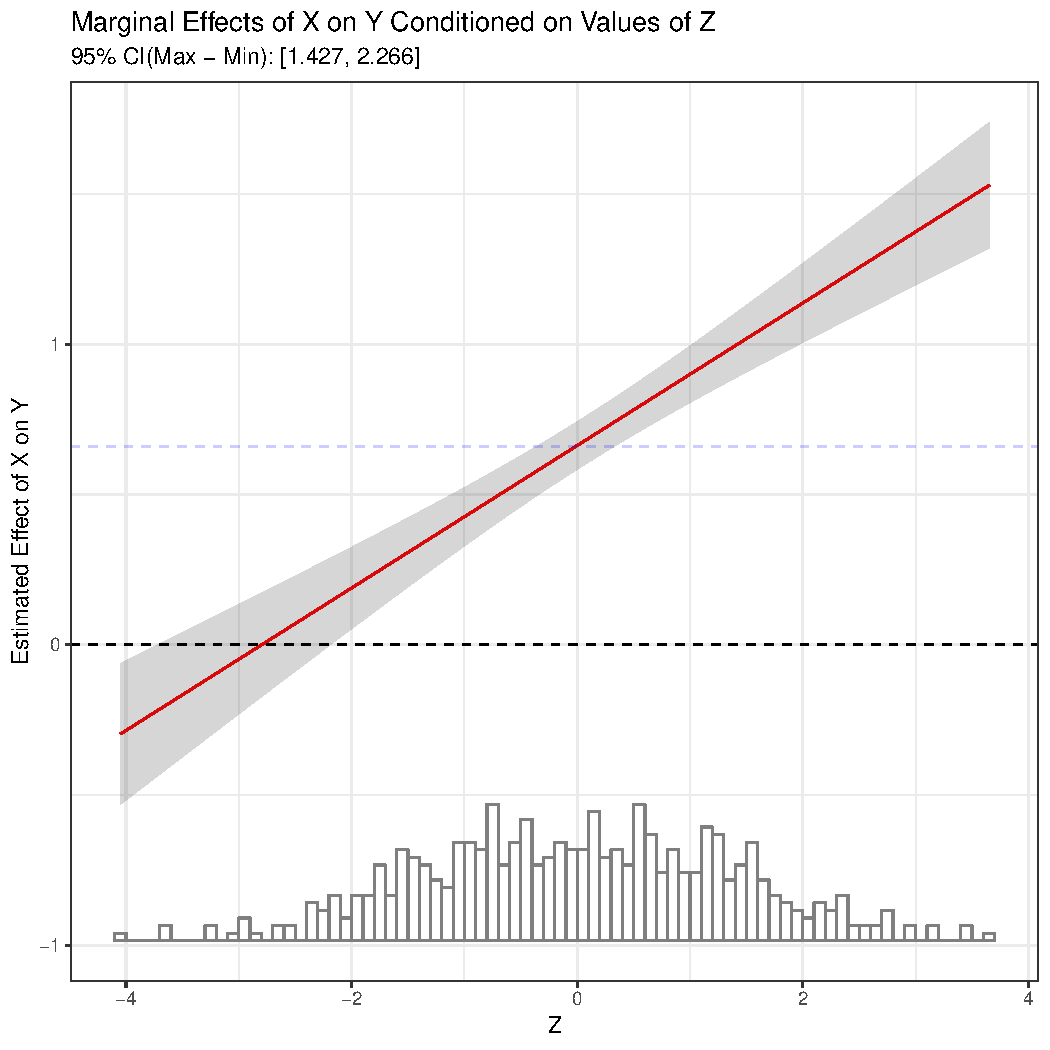
\includegraphics[scale=.6]{images/cond0.pdf}
    \caption{Conditional marginal effects of $X$ on $Y$ across values of $Z$. The red line represents the estimated marginal effects, with the gray bands being $95\%$ confidence intervals. The faint blue line at $Y = .66$ shows the estimated marginal effect when the interaction term is not included in the model.}
    \label{fig:cond0}
\end{figure}

Figure \ref{fig:cond0} helps us gain a more comprehensive understanding of how $Z$ moderates the effect of $X$ on $Y$. First, as per equations \ref{mod} and \ref{mod2}, the unstandardized estimate of the interaction effect is equal to the slope of the line observed in the plot $(\hat{\beta}_3 = 0.24)$. Additionally, the marginal effect conditioned on $Z = 0$ is equal to the unstandardized main effect of $X$ on $Y$ $(\hat{\beta}_1 = 0.66)$. The gray bands surrounding the marginal effects represent $95\%$ confidence intervals based on the standard errors estimated from equation \ref{margse}. We can see that the intervals do not include $0$ over most the range of $Z$, and reveal that $X$ is expected to have a significant \textit{negative} effect on $Y$ at low values of $Z$, but a significant \textit{positive} effect across the majority of $Z$'s range. Moreover, the histogram at the bottom of the plot displays the distribution of $Z$, and the $95\%\ \text{CI}$ at the top represents the difference between effects estimated at its maximum and minimum using data simulated from the posterior distribution of $(\hat{\beta}_1 + \hat{\beta}_3 Z)$ with the \code{sim} function from the \code{arm} package in R \cite{arm}. 

\subsubsection{Discussion}
The purpose of this example is to demonstrate how a researcher might go about probing an interaction effect by examining the conditional effects of an independent variable across the range of a continuous moderator. Importantly, this plot illustrates the necessity of testing interaction effects when one is investigating a conditional hypothesis. Although this is a simulated example, we can clearly see that without modeling the interaction between $X$ and $Z$, one's understanding of the relationship between $X$ and $Y$ would be greatly misrepresented. Had the interaction effect not been included, the estimated marginal effect of $X$ on $Y$ would be captured by the dashed blue line where the $y$-axis equals $0.66$. This is the main effect of $X$ on $Y$ in the non-interaction model, where $Z$ is still included as a covariate. The bottom line is that visualizing the character of how two variables interact is crucial for understanding how they might relate with an outcome of interest. Especially for multivariate models such as psychological networks, failing to include relevant interaction terms can lead to misspecified models that improperly characterize the relationships among a set of variables. This plotting function is included as part of the \code{modnets} package for assessing interaction effects within psychological network models; thus, it is a tool that researchers studying moderated networks in psychology will be able to use as part of their analyses and profitably employ to explore the nature of interaction effects in their models. 

\subsection{Summary}
The goal of the present section was to provide a background describing moderation analysis, interaction effects, and how rich information about multivariate relationships can be gained from studying the conditional effects of a given predictor on an outcome after considering values of a moderator. The central point here was to showcase a simple way of extracting this type of information from a moderated regression model to better understand the nature of the relationships among variables.

In the next section, I will present my approach to analyzing \textit{moderated network models}, which are essentially a multivariate generalization of the basic template presented here. Combined with techniques from graphical modeling, adding interaction terms to network models contributes a potentially powerful framework for investigating more complex models and more specific hypotheses (namely, those dealing with moderation and interaction effects). Furthermore, generalizing the concept of plotting conditional effects across values of a moderator, I will present a new contribution to psychological network modeling which I term \textit{conditional networks}. As in the case of plotting marginal effects at specific values of a moderator, I will show how we can construct networks after conditioning on specific values of a moderator. This offers a way of gaining added information about moderated networks and visualizing the results in easily interpretable plots. I present the basic ideas behind moderated networks in the next section.
